\chapter{B-tree, 23-tree, 234-tree, RB-tree}

\lecture{10}{28 Nov. 14:20}{}

\section{RB-tree}

\begin{definition}[RB-tree]
    RB-tree (Red-Black tree) --- binary search tree with additional properties:
    \begin{itemize}
        \item For black node, 
        \begin{enumerate}[label=(\arabic*)]
            \item Root is black.
            \item All paths from leaf to root contain the same number of black nodes.
        \end{enumerate}
        \item For red node, 
        \begin{enumerate}[label=(\arabic*)]
            \item No red node has a red child.
        \end{enumerate}
        \item BST property holds.
        \begin{enumerate}[label=(\arabic*)]
            \item Every non-leaf node have two children.
            \item The whole tree are increasing in in-order traversal.
        \end{enumerate}
    \end{itemize}
\end{definition}

\begin{figure}[H]
    \centering
    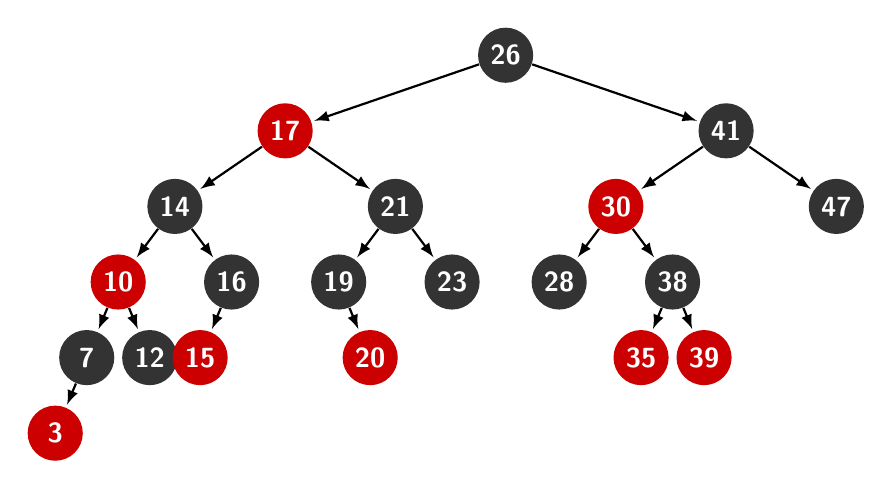
\begin{tikzpicture}[
        % --- 區域樣式設定 ---
        every node/.style={circle, text=white, minimum size=7mm, inner sep=0pt, font=\sffamily\bfseries},
        bn/.style={fill=black!80},       % 黑色節點
        rn/.style={fill=red!80!black},   % 紅色節點
        level 1/.style={sibling distance=70mm},
        level 2/.style={sibling distance=35mm},
        level 3/.style={sibling distance=18mm},
        level 4/.style={sibling distance=10mm},
        level distance=1.2cm,
        edge from parent/.style={draw, ->, thick, >=latex, shorten >=1pt},
        % --------------------
        scale=0.8
    ]

    % 根節點 26 (黑)
    \node[bn] {26}
        % --- 左子樹 ---
        child { node[rn] {17}
        child { node[bn] {14}
            child { node[rn] {10}
            child { node[bn] {7}
                child { node[rn] {3} }
                child[missing] 
            }
            child { node[bn] {12} }
            }
            child { node[bn] {16}
            child { node[rn] {15} }
            child[missing] 
            }
        }
        child { node[bn] {21}
            child { node[bn] {19}
            child[missing] 
            child { node[rn] {20} }
            }
            child { node[bn] {23} }
        }
        }
        % --- 右子樹 ---
        child { node[bn] {41}  % 修正:依圖示應為黑色
        child { node[rn] {30} % 修正:依圖示應為紅色
            child { node[bn] {28} }
            child { node[bn] {38}
            child { node[rn] {35} }
            child { node[rn] {39} }
            }
        }
        child { node[bn] {47} }
        };
    \end{tikzpicture}
    \caption{An example of RB-tree}
\end{figure}

\begin{note}
    The height of RB-tree with $n$ nodes is $O(\log n)$, which is use to guarantee the time complexity of search, insert and delete operation is $O(\log n)$ with balancing the tree.
\end{note}

\section{Balance Tree (B-tree)}

\begin{definition}[B-tree]
    B-tree of order $t$ is a tree with the following properties:
    \begin{itemize}
        \item Every node has at most $t$ children.
        \item Every non-leaf node (except root) has at least $\lceil t/2 \rceil$ children.
        \item A non-leaf node with $k$ children contains $k-1$ keys.
        \item All leaves appear on the same level.
        \item The keys in each node are sorted in increasing order.
    \end{itemize}
\end{definition}

\begin{definition}[23-tree]
    23-tree is a B-tree of order 3.
\end{definition}

\begin{definition}[234-tree]
    234-tree is a B-tree of order 4.
\end{definition}
\begin{note}
    The height of B-tree with $n$ nodes is $O(\log n)$, which is use to guarantee the time complexity of search, insert and delete operation is $O(\log n)$ with balancing the tree.
\end{note}

\begin{remark}
    We can convert RB-tree to 234-tree by merging red nodes to their black parent nodes in $O(n)$, which means they are equivalent in terms of search, insert and delete operations.
\end{remark}

\begin{figure}[H]
    \centering
    \begin{tikzpicture}[
      % --- 設定 ---
      level distance=1.5cm,
      % 第一層兄弟距離要拉大,避免重疊
      level 1/.style={sibling distance=50mm},
      % 第二層兄弟距離縮小
      level 2/.style={sibling distance=20mm},
      edge from parent/.style={draw, -Latex, thick},
      % --- B-Tree 節點樣式 ---
      % #1 = 格子數量 (keys 數量)
      btnode/.style={
        draw,
        rectangle split,
        rectangle split horizontal,
        rectangle split parts=#1, 
        fill=white,
        rounded corners=3pt,
        minimum height=2.2em,
        font=\bfseries\sffamily
      }
    ]
    
      % --- 根節點 [17 | 26] ---
      % 來源:黑節點 26 + 左紅子 17
      \node[btnode=2] {17 \nodepart{two} 26}
        % --- 左子 (對應 < 17) ---
        % 來源:黑節點 14 + 左紅子 10
        child { 
          node[btnode=2] {10 \nodepart{two} 14}
            % 子節點 < 10 (7+3)
            child { node[btnode=2] {3 \nodepart{two} 7} }
            % 子節點 10~14 (12)
            child { node[btnode=1] {12} }
            % 子節點 > 14 (16+15)
            child { node[btnode=2] {15 \nodepart{two} 16} }
        }
        % --- 中子 (對應 17 ~ 26) ---
        % 來源:黑節點 21
        child { 
          node[btnode=1] {21}
            % 子節點 < 21 (19+20)
            child { node[btnode=2] {19 \nodepart{two} 20} }
            % 子節點 > 21 (23)
            child { node[btnode=1] {23} }
        }
        % --- 右子 (對應 > 26) ---
        % 來源:黑節點 41 + 左紅子 30
        child { 
          node[btnode=2] {30 \nodepart{two} 41}
            % 子節點 < 30 (28)
            child { node[btnode=1] {28} }
            % 子節點 30~41 (38+35+39) --> 這是一個 3 keys 節點
            child { node[btnode=3] {35 \nodepart{two} 38 \nodepart{three} 39} }
            % 子節點 > 41 (47)
            child { node[btnode=1] {47} }
        };
    
    \end{tikzpicture}
    \caption{Convert RB-tree to 234-tree}
\end{figure}

\newpage

\begin{note}
    To convert RB-tree to 23-tree, we can follow the same procedure as converting to 234-tree, but we need to ensure we always combine the right child red node with its black parent node.
\end{note}

\begin{figure}[H]
    \centering
    \begin{tikzpicture}[
      % --- 設定 ---
      level distance=1.5cm,
      % 根節點到第一層的距離
      level 1/.style={sibling distance=70mm},
      % 第一層到第二層的距離
      level 2/.style={sibling distance=35mm},
      % 底層葉子之間的距離 (需要微調以防重疊)
      level 3/.style={sibling distance=15mm},
      edge from parent/.style={draw, -Latex, thick},
      % --- B-Tree 節點樣式 (2-3 Tree 只有 1 key 或 2 keys) ---
      btnode/.style={
        draw,
        rectangle split,
        rectangle split horizontal,
        rectangle split parts=#1, 
        fill=white,
        rounded corners=3pt,
        minimum height=2.2em,
        font=\bfseries\sffamily
      },
      scale=0.8
    ]
      % --- Level 0: 新的根節點 ---
      % 因為 [17, 26, 38] 分裂,26 被推到最頂端
      \node[btnode=1] {26}
        % --- Level 1: 左子樹 (由 17 領軍) ---
        child { 
          node[btnode=1] {17}
            % Level 2
            child { 
              node[btnode=2] {10 \nodepart{two} 14} 
                % Level 3 Leaves
                child { node[btnode=2] {3 \nodepart{two} 7} }
                child { node[btnode=1] {12} }
                child { node[btnode=2] {15 \nodepart{two} 16} }
            }
            child { 
              node[btnode=1] {21}
                 % Level 3 Leaves
                child { node[btnode=2] {19 \nodepart{two} 20} }
                child { node[btnode=1] {23} }
            }
        }
        % --- Level 1: 右子樹 (由 38 領軍) ---
        % 38 是從底層一路被擠上來的
        child { 
          node[btnode=1] {38}
            % Level 2
            child { 
              node[btnode=1] {30}
                % Level 3 Leaves
                child { node[btnode=1] {28} }
                child { node[btnode=1] {35} } % 35 從原來的 [35,38,39] 分裂出來
            }
            child { 
              node[btnode=1] {41}
                % Level 3 Leaves
                child { node[btnode=1] {39} } % 39 從原來的 [35,38,39] 分裂出來
                child { node[btnode=1] {47} }
            }
        };
    \end{tikzpicture}
    \caption{Convert RB-tree to 23-tree}
\end{figure}


\chapter{Hashing, Randomized Algorithm \& Communication Complexity}

\section{Hashing}

\begin{exercise}
    Suppose that we want to represent an initially empty set $S$ of at most $n$
    numbers such that each element of $S$ is a positive integer no more than
    $n$. We would like to support the following operations on $S$ for any given
    integer $i$ with $1 \leq i \leq n$:
    \begin{itemize}
        \item membership: determining whether $i$ belongs to $S$.
        \item insertion: inserting $i$ into $S$.
        \item deletion: deleting $i$ from $S$.
    \end{itemize}
\end{exercise}

To implement the above operations alll in $O(1)$ time, we can use an array of size $n$ (let's call it `A') initialized to all zeros. Each index of the array corresponds to an integer from $1$ to $n$.

\begin{intuition}
    We can use a sorted array or a balanced search tree to store the elements of $S$. However, both approaches would require $O(\log n)$ time for membership, insertion, and deletion operations. But it may be possible to achieve $O(1)$ time.
\end{intuition}

\begin{idea}
    Keep all the elements of $S$ in a \textcolor{red}{binary} array $C[1 \dots, n]$. Specifically, for each $j = 1, \dots, n$, we maintain the condition that $C[j] = 1$ holds if and only if $S$ contains element $j$.
    
    \begin{itemize}
        \item Space: $O(n)$.
        \item Time:
        \begin{itemize}
            \item creation and initialization: $O(n)$.
            \item membership: $O(1)$ (direct look-up).
            \item insertion: $O(1)$.
            \item deletion: $O(1)$.
        \end{itemize}
    \end{itemize}
\end{idea}

\begin{remark}
    This method still requires $O(n)$ for initialization time.
\end{remark}

\begin{idea}
    Maintain a \textcolor{red}{dense} array $D[1 \dots n]$ storing the elements contiguously, a \textcolor{red}{sparse} array $S[1 \dots U]$, and a size counter $k$. 
    The condition that $x \in Set$ holds if and only if $1 \le S[x] \le k$ and $D[S[x]] = x$.
    
    \begin{itemize}
        \item Space: $O(n)$ (requires memory for the universe size).
        \item Time:
        \begin{itemize}
            \item creation and initialization: $O(1)$ (\textbf{no need to zero out arrays}).
            \item membership: $O(1)$ (via double-check logic).
            \item insertion: $O(1)$.
            \item deletion: $O(1)$.
        \end{itemize}
    \end{itemize}
\end{idea}

\vspace{1em}

If we want to store a set of $n$ numbers are all integers in the range $1$ to $m$ where $m$ is much larger than $n$, the above methods would be inefficient in terms of space. If we can have a finger printing function that maps the large universe of size $m$ to a smaller range of size $O(n)$, we can then use the above methods to store the set efficiently.

\begin{intuition}
    We want to find a function that maps a large universe of size $m$ to a smaller range of size $O(n)$ in $O(1)$ time.
    \[
        H: \{1, 2, \dots, m\} \to \{1, 2, \dots, k\} \quad \text{where } k = O(n)
    \]
    where \[
        \forall x \neq y, H(x) \neq H(y)
    \]
\end{intuition}

\section{Randomized Algorithm \& Communication Complexity}

\begin{exercise}
    Given
    \begin{itemize}
        \item Input: two $n \times n$ matrices $A$ and $B$.
        \item Output: determine whether $A = B$
    \end{itemize}
\end{exercise}
\begin{com}[1]
    The time complexity is $\Theta(n^2)$ by checking each entry one by one.
\end{com}
\begin{com}[2]
    But we are more interested in communication complexity. To minimize the communication between two parties (Alice and Bob), we can use a randomized algorithm.
\end{com}

\begin{idea}
    We can use the following randomized algorithm:
    \begin{itemize}
        \item Alice and Bob agree on a vector $r$ with $n$ entries where each entry is chosen uniformly at random from $\{0,1\}$.
        \item Compare the vectors $Ar$ and $Br$.
    \end{itemize}
\end{idea}

\begin{com}
    The communication complexity of this algorithm is $O(n)$ if we don't count the initial agreement on $p$.
\end{com}

We can do some analysis on the error probability of this algorithm. If $A = B$, then $Ar = Br$ always holds. If $A \neq B$, we want to bound the probability that $Ar = Br$.

\begin{proposition}
    \[
        \Pr[Ar = Br \mid A = B] = 1 \tag{1}
    \]
    \[
        \Pr[Ar = Br \mid A \neq B] \leq 0.5 \tag{2}
    \]
\end{proposition}
\begin{proof}
    Equation (1) is trivial. For Equation (2), let $C = A - B$. Since $A \neq B$, we can show that \[
        \Pr[Cr = 0^n \mid C\neq 0^{n \times n} ] \leq 0.5
    \]
    Assuming $C \neq 0^{n \times n}$, there is a row $i$ of $C$ whose nonzero entries are $c_{i1}, c_{i2}, \dots, c_{ik}$ for a $k \geq 1$. Thus, it suffices to show that \[
        \Pr\left[\sum_{j=1}^{k} c_{ij_k} r_{j_k} = 0 \middle| c_{ij} \neq 0 \text{ for some } j\right] \leq 0.5
    \]
    Let $r_{j_k}$ be the last random variable in the summation. When all the other elements of $r$ determined, at most one choice of $r_{j_k}$ can satisfy the equation. \[
        \sum_{j=1}^{k} C_{ij_k} r_{j_k} = 0 \implies r_{j_k} = -\frac{\sum_{j=1}^{k-1} c_{ij_k} r_{j_k}}{c_{ij_k}}
    \]
    Thus, the probability is at most $0.5$.
\end{proof}

If we think about the error probability is too high, we have two solutions:

\begin{idea}
    We can repeat the above algorithm $t = O(1)$ to reduce the error probability to $2^{-t}$ but the communication complexity would increase to $O(tn) = O(n)$.
\end{idea}

\begin{idea}
    We can use the following randomized algorithm:
    \begin{itemize}
        \item Alice and Bob agree on a large prime number $p$ (e.g., $p > n^2$).
        \item Alice randomly selects a vector $r \in \mathbb{Z}_p^n$ where each entry is chosen uniformly at random from $\{0, 1, \dots, p-1\}$.
        \item Alice computes the vector $Ar$ and sends it to Bob.
        \item Bob computes the vector $Br$ and compares it with the received vector $Ar$.
        \item If $Ar = Br$, Bob concludes that $A = B$; otherwise, he concludes that $A \neq B$.
    \end{itemize}
\end{idea}

\chapter{P \& NP}

\section{P-class \& NP-class}

\begin{definition}[P-class]
    P-class is the class of decision problems that can be solved by a deterministic Turing machine in polynomial time.
\end{definition}

\begin{definition}[NP-class]
    NP-class is the class of decision problems for which a given solution can be verified by a deterministic Turing machine in polynomial time. Or equivalently, NP-class is the class of decision problems that can be solved by a non-deterministic Turing machine in polynomial time.
\end{definition}

\begin{remark}
    To see the definition of deterministic and non-deterministic Turing machine, please refer to the note on Introduction to the Theory of Computation (CSIE 3110) or the note I made.
\end{remark}

\begin{exercise}
    Given
    \begin{itemize}
        \item Input: a graph $G$ and an integer $k$.
        \item Output: determine whether $G$ contains a clique of size $k$.
    \end{itemize}
\end{exercise}

\begin{idea}[Non-deterministic Algorithm for Clique Problem]
    Let set S be the empty vertex set. For each vertex $x$ of $G$, (non-deterministically) either insert $x$ into $S$ or do nothing. If $|S| \leq k$ and $S$ is a vertex cover of $G$, then output yes. Otherwise, output no.
\end{idea}

\begin{note}[Correctness of Non-deterministic Algorithm]
    The correctness of the non-deterministic algorithm should be checked by
    \begin{itemize}
        \item If YES, then there is a computation path of the algorithm that leads to yes.
        \item If NO, then all computation paths of the algorithm lead to no.
    \end{itemize}
\end{note}

\begin{note}[Time Complexity of Non-deterministic Algorithm]
    We say that a nondeterministic algorithm $N$ runs in polynomial time if for any input $x$ of $N$, any computation of $N$ on $x$ takes time polynomial in the size of $x$.
\end{note}

\newpage

We have more type then we can discuss about P-class and NP-class.
\begin{itemize}
    \item P-class $\subseteq$ NP-class.
    \item Each NP problem can be solved by a deterministic Turing machine in exponential time.
    \item If $P = NP$, then all NP problems can be solved by a deterministic Turing machine in polynomial time.
    \item Whether $P = NP$ or not is still an open problem.
    \begin{itemize}
        \item $P = NP$: All hardest problems in NP can be solved in polynomial time.
        \item $P \neq NP$: There are some problems in NP that cannot be solved in polynomial time.
    \end{itemize}
\end{itemize}